\section{A model of human behavior for \ac{WCA}}\label{sec:model}


In order to accurately emulate the behavior of a human, a model for \ac{WCA} needs to implement two main behaviors.
One, it needs to generate realistic execution times for each step in the task, considering the current and historical impairment of the \ac{WCA} system.
We detail this in \cref{ssec:model:exectimes}.
And two, it needs to produce sequences of input samples for each step mimicking what a real human would generate; this is explained in \cref{ssec:model:frames}.

In the following subsections, \cref{ssec:model:exectimes,ssec:model:frames}, we explain how we design a model which fulfills these requirements.
We briefly discuss where implementations of this model can be obtained in \cref{ssec:model:impl}

\subsection{Generating realistic execution times}\label{ssec:model:exectimes}

As expressed in \cref{ssec:plos}, for ~\cite{olguinmunoz:impact2021} we collected timing and task performance data for \num{40} participants performing a \num{169}-step task, guided by a \ac{WCA}, as well as personality trait scores for each participant.
For this paper, we use this data to construct a probabilistic model for the generation of realistic execution times.
The data is pre-processed to group execution time values by level of neuroticism, previous \acp{TTF}, and duration of impairment.
The resulting collections of execution times represent the distributions of these values for users with specific levels of neuroticism, interacting with systems at specific states of impairment and recent histories of impairment.
These distributions can then be sampled to produce new, realistic execution times.
In the following, we detail the step-by-step processing of this data and construction of the probabilistic model.

\begin{table}
\centering
\caption[A]{%
    Sample of the execution time data  used for the elaboration of the timing model.
    Rows contain the execution times and \acp{TTF} for each of the \num{169} steps performed by the \num{40} participants in \textcite{olguinmunoz:impact2021}, expressed in seconds, together with a unique identifier for the subject, their associated level of normalized neuroticism, and a sequence number identifying the position of the step in the task.
}\label{tab:data:exectime}
\begin{tabular}{rrrrrr}
    \toprule
    {seq} & {run\_id} & {exec\_time} & {ttf} & {neuroticism}\\
    \midrule
    1 & 134146 & 3.655 & 0.597 & 0.375\\
    2 & 134146 & 4.439 & 0.554 & 0.375\\
    3 & 134146 & 2.943 & 0.562 & 0.375\\
    \( \cdots \) & \( \cdots \) & \( \cdots \) & \( \cdots \) & \( \cdots \) \\
    169 & 134146 & 3.532 & 4.571 & 0.375\\
    1 & 134470 & 3.461 & 0.561 & 0.594\\
    2 & 134470 & 6.678 & 0.572 & 0.594\\
    \( \cdots \) & \( \cdots \) & \( \cdots \) & \( \cdots \) & \( \cdots \) \\
    \( \cdots \) & \( \cdots \) & \( \cdots \) & \( \cdots \) & \( \cdots \) \\
    169 & 137353 & 4.615 & 0.537 & 0.625\\
    \bottomrule
    \end{tabular}
\end{table}

We employ a cleaned and re-parameterized copy of the aforementioned timing data.
The \num{6760} data points are arranged in a table, a sample of which can be seen in \cref{tab:data:exectime}, together with identifiers for the subjects, their neuroticism score, and a sequence number for each step.

\begin{table}[]
\centering
\caption{%
    Default bins used for model parameter levels.
    For impairment, values were rounded to three decimal places.
}
\label{tab:defaultbins}
% \resizebox{\columnwidth}{!}{%
\begin{tabular}{@{}lccc@{}}
\toprule
\textbf{Parameter} & \textbf{Low}     & \textbf{Medium}      & \textbf{High}         \\ \midrule
Neuroticism        & \( [0, 0.5) \)   &                      & \( [0.5, 1.0] \)      \\
Impairment         & \( [0, 1.482) \) & \( [1.482, 3.198) \) & \( [3.198, \infty) \) \\
Duration           & \( [0, 5) \)     & \( [5, 10) \)        & \( [10, \infty) \)    \\ \bottomrule
\end{tabular}%
% }
\end{table}

We begin by discretizing normalized neuroticism into \emph{low} and \emph{high} ranges, and \ac{TTF} into three ranges by splitting the data on the 3-quantiles; we will refer to these ranges of \ac{TTF} as \emph{low}, \emph{medium}, and \emph{high impairment}.
\cref{tab:defaultbins} shows the exact values used for these ranges.

The next steps of processing are slightly more complex.
For the data of each subject (which we will refer to as a \emph{run}), we shift the execution times by one sample such that each \ac{TTF} measurement (and therefore, impairment level) is associated with the execution time for the next step.
This comes directly from our discussions in \cref{sec:background} and~\cite{olguinmunoz:impact2021}.
Users notice the impairment of the current step only when they have finished it, and thus system impairment has no effect on the execution time of the current step, but directly affects the next one.

We then assign a label to each sample indicating the class of the most recent transition in impairment level in the run.
In other words, for each recorded step, we look back until we find a step with a different level of impairment and assign a label to the current step according to whether that change was from a higher to a lower level of impairment or vice-versa.
However, if the current step is too far from the latest transition in impairment (by default, more than \num{8} steps), it is instead marked as \emph{no transition}; this label is also used for steps at the beginning of each run which have no previous transition in impairment.
This labeling allows us to capture the behavior described in \cref{item:remain} of \cref{ssec:plos}.

Finally, we assign a number to each sample corresponding to \emph{how long} the current combination of level of impairment and transition has been in effect, in number of steps.
This count resets whenever this combination changes.
This value is subsequently discretized into three levels; \emph{short}, \emph{medium}, and \emph{long duration} (again, refer to \cref{tab:defaultbins} for the exact values used).

The results of this processing on the samples from \cref{tab:data:exectime} can be seen in \cref{tab:data:exectime:processed}.
Three examples of the effect of this discretization and processing on the data are also presented in \cref{fig:timing}.
Specifically, we showcase how
\begin{enumerate*}[itemjoin={{; }}, itemjoin*={{; and}}]
    \item higher neuroticism leads to higher mean execution times as impairment goes up (\cref{fig:timing:impneurvsetime})
    \item duration has both a speed-up and slow-down effect on execution times, depending on the level of impairment (\cref{fig:timing:durvsetime})
    \item transitions from higher to lower levels of impairment lead to higher mean execution times when compared to steps far away from a transition, or from a transition from lower to higher levels of impairment (\cref{fig:timing:imptransvsetime})
\end{enumerate*}.


Finally, in \cref{alg:timings} we present a step-by-step breakdown of how this data is subsequently used to generate realistic execution times.
In plain English, a model which uses this processed data to generate execution times needs to maintain variables for duration, previous impairment, and most recent transition.
At the beginning of each step, the model
\begin{enumerate}
    \item Checks whether any change in impairment has occurred.
    If it has, it resets duration to \num{1} and updates the transition variable accordingly.
    If not, it increases the duration variable by one unless that increase causes it to exceed the threshold of steps required to forget a transition.
    If that's the case, instead the model resets duration to \num{1} and sets the transition variable to ``no transition''.
    \item Discretizes the updated duration value.
    \item Finds all samples with binned neuroticism, impairment, duration, and transition values matching the current state of the system.
    \item Randomly samples the filtered data to obtain a realistic execution time value.
    \begin{itemize}
        \item Alternatively, a distribution can be first be fitted to the filtered samples.
        The model then samples the theoretical distribution instead of the empirical samples.
    \end{itemize}
    \item Finally, updates the stored impairment value with the new impairment and proceeds to the next step.
\end{enumerate}

\begin{algorithm}
    \caption{Generating realistic execution times}\label{alg:timings}

    \SetKwInput{KwState}{Initial State}

    \KwIn{$\tau$: \ac{TTF} of the previous step.}
    \KwOut{$t_\text{exec}$: next execution time.}
    \KwState{%
        \begin{itemize}
            \item Binned neuroticism $N$.
            \item Number of steps to remember transitions for: $\delta \leftarrow 8$.
            \item Duration counter: $d \leftarrow 0$.
            \item Previous impairment: $I' \leftarrow \varnothing$.
            \item $B_\text{TTF}$ and $B_\text{duration}$ are functions for binning \ac{TTF} and duration into discrete levels, respectively.
            \item $F_\text{data}$ is a function which filters the data and returns only execution time samples which match the given levels of binned neuroticism, binned impairment, binned duration, and transition label.
        \end{itemize}
    }

    $I \leftarrow B_\text{TTF}(\tau)$ \tcc*{discretize \ac{TTF}}

    \uIf{($I' == \varnothing$) {\normalfont\textbf{or}}\\\hspace{1em}($T \neq \text{``NO TRANSITION''}$ {\normalfont\textbf{and}} $d + 1 > \delta$)}{%
        $d \leftarrow 1$\;
        $T \leftarrow \text{``NO TRANSITION''}$\;
    } \uElseIf{$I' < I$}{%
        $d \leftarrow 1$\;
        $T \leftarrow \text{``LOWER TO HIGHER''} $
    } \uElseIf{$I' > I$}{%
        $d \leftarrow 1$\;
        $T \leftarrow \text{``HIGHER TO LOWER''} $  
    } \Else {%
        $d \leftarrow d + 1$\;
    }
    $I' \leftarrow I$ \tcc*{store impairment for later}
    $D \leftarrow B_\text{duration}(d)$ \tcc*{discretize duration}

    \tcc{next, filter the data to select only the matching samples}
    $E \leftarrow F_\text{data}(N, I, D, T)$ \;
    \tcc{finally, sample the data to return a realistic execution time}
    $t_\text{exec} \leftarrow {SAMPLE}(E)$\;

\end{algorithm}


\begin{table*}
\caption{Sample of the processed execution time data table.}\label{tab:data:exectime:processed}
\begin{tabular}{rrrrcrccrc}
\toprule
{seq} & {run\_id} & {next\_exec\_time} & {ttf} & {impairment} & {neuroticism\_raw} & {neuroticism} & {transition} & {duration\_raw} & {duration} \\
\midrule
1   & 134146 & 3.655 & 0.000 & low & 0.375  & low & NoTransition & 1 & short \\
2   & 134146 & 4.439 & 0.597 & low & 0.375 & low & NoTransition & 2 & short \\
3   & 134146 & 2.943 & 0.554 & low & 0.375 & low & NoTransition & 3 & short \\
\( \cdots \) & \( \cdots \) & \( \cdots \) & \( \cdots \) & \( \cdots \) & \( \cdots \) & \( \cdots \) & \( \cdots \) & \( \cdots \) & \( \cdots \)\\
169 & 134146 & 3.532 & 3.689 & high & 0.375 & low & Lower2Higher & 2 & short \\
1   & 134470 & 3.461 & 0.000 & low & 0.594 & high & NoTransition & 1 & short \\
2   & 134470 & 6.678 & 0.561 & low & 0.594 & high & NoTransition & 2 & short \\
\( \cdots \) & \( \cdots \) & \( \cdots \) & \( \cdots \) & \( \cdots \) & \( \cdots \) & \( \cdots \) & \( \cdots \) & \( \cdots \) & \( \cdots \)\\
\( \cdots \) & \( \cdots \) & \( \cdots \) & \( \cdots \) & \( \cdots \) & \( \cdots \) & \( \cdots \) & \( \cdots \) & \( \cdots \) & \( \cdots \)\\
169 & 137353 & 4.615 & 0.579 & low & 0.625 & high & NoTransition & 2 & short \\
\bottomrule
\end{tabular}
\end{table*}

\begin{figure*}
    \centering
    \begin{subfigure}[t]{.28\textwidth}
        \centering
        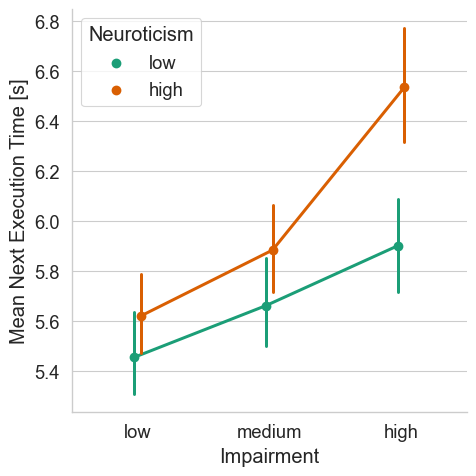
\includegraphics[width=\textwidth]{./model_data/imp_neur_vs_exectime.png}
        \caption{}\label{fig:timing:impneurvsetime}
    \end{subfigure}%
    \hspace{.05\textwidth}%
    \begin{subfigure}[t]{.28\textwidth}
        \centering
        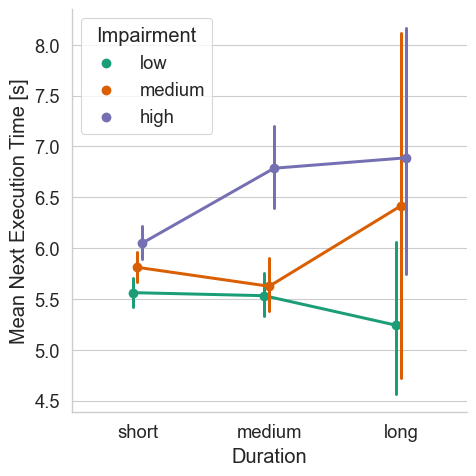
\includegraphics[width=\textwidth]{./model_data/duration_vs_exectime.png}
        \caption{}\label{fig:timing:durvsetime}
    \end{subfigure}%
    \hspace{.05\textwidth}%
    \begin{subfigure}[t]{.28\textwidth}
        \centering
        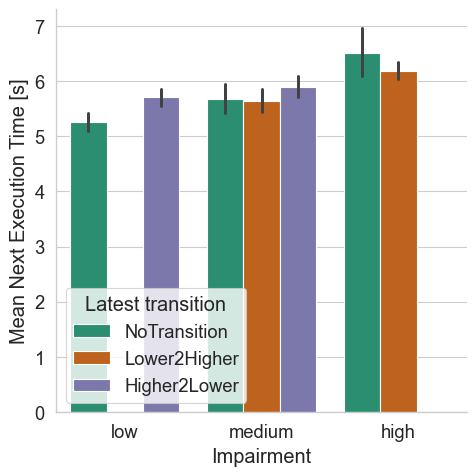
\includegraphics[width=\textwidth]{./model_data/impairment_transition_vs_exectime.png}
        \caption{}\label{fig:timing:imptransvsetime}
    \end{subfigure}
    \caption{%
        Visualizations of the model data after discretization and post-processing.
        \subref{fig:timing:impneurvsetime} illustrates the effect of impairment on execution times, and how neuroticism modulates this behavior;
        \subref{fig:timing:durvsetime} exemplifies how the model captures the speed-up and slow-down behaviors due to impairment and duration described in \textcite{olguinmunoz:impact2021};
        finally, \subref{fig:timing:imptransvsetime} shows the lingering effects of impairment after a transition.
    }\label{fig:timing}
\end{figure*}

\subsection{Generating realistic samples}\label{ssec:model:frames}

Apart from the aforementioned timing and performance data, for~\cite{olguinmunoz:impact2021} we also recorded all collected video frame samples together with matching metadata.
For each video frame submitted to the \ac{WCA} during the tasks, we recorded
\begin{enumerate*}[itemjoin={{; }}, itemjoin*={{; and }}]
    \item the raw video frame captured
    \item sample submission timestamp
    \item \ac{WCA} processing completed timestamp
    \item result or acknowledgement returned timestamp
    \item a tag representing the result of the \ac{WCA} processing
\end{enumerate*}.
The tags assigned corresponded to:
\begin{description}[font={\bfseries\ttfamily}]
    \item[SUCCESS:] frames which triggered a transition to a new step in the logical task model of the \ac{WCA}, and thus cause the generation of feedback to the user.
    This tag is also used for frames which corrected a previous mistake.
    \item[REPEAT:] frames which contained the same board state as the previous successful frame, and thus produced no feedback.
    \item[LOW\_CONFIDENCE] frames for which the image recognition algorithm in the \ac{WCA} did not reach the necessary confidence threshold to interpret it as a valid board state.
    These frames also produce no feedback.
    \item[BLANK] frames in which not enough of the board is visible due to noise, movement, occlusion, etc.
    These frames produce no feedback either.
    \item[TASK\_ERROR] frames which contained an incorrect board state and thus triggered a transition to a procedural corrective step and the generation of feedback to the user.
    However, it must be noted that none of the \num{40} participants made any mistakes during the task, and thus no such frames were encountered in the data.
\end{description}

We correlate this frame data with the step timing data described in \cref{ssec:model:exectimes} to match frames with their corresponding step execution times.
We assign to each frame a normalized instant value corresponding to its capture instant (expressed in seconds since the start of the step) divided by the total execution time of the step.
To exemplify, for a step with execution time \( t_\text{exec} = \SI{10}{\second} \), a frame captured at time \( \tau = \SI{3}{\second} \) from the start of the step, will have a normalized instant value \( t_\text{norm} \):
\begin{align}
    t_\text{norm} = \frac{\tau}{t_\text{exec}} = \frac{\SI{3}{\second}}{\SI{10}{\second}} = 0.3
\end{align}

This allows us to then analyze the distribution of frame tag probabilities as a step progresses, independently of execution times.
This is illustrated in \cref{fig:frameprobs}. 
Intuitively, \texttt{REPEAT} frames dominate the early instants after a step transition, as the user has not had time to start performing the new instruction and thus the \ac{WCA} keeps capturing frames representing the previous state of the board.
As the user starts moving and performing actions, \texttt{BLANK} frames start to dominate, as this activity prevents the \ac{WCA} from capturing ``clean'' frames.
Finally, it must be noted that \texttt{SUCCESS} frames are not included in this probability density plot, as, by definition (\( t_\text{norm} \) represents the normalized instant value):
\begin{equation}
    P(\text{\texttt{SUCCESS}} | t_\text{norm}) =
    \left\{ \begin{array}{ll}
        0 & t_\text{norm} < 1.0 \\
        1 & t_\text{norm} \geq 1.0    
    \end{array} \right.
\end{equation}
That is, any frame captured immediately at or after the execution time has been reached will contain the finished board state and thus correspond to a \texttt{SUCCESS} frame.

\begin{figure}
    \centering
    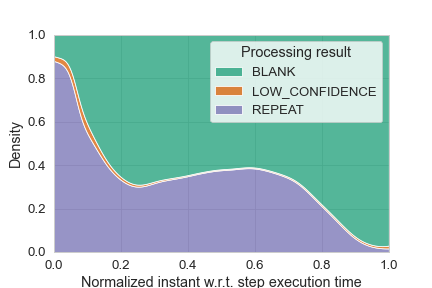
\includegraphics[width=\columnwidth]{model_data/frame_probabilities.png}
    \caption{%
        Probability density of frame result tags as a step progresses.
        Note that \texttt{SUCCESS} frames are not included as --- by definition --- the probability for success frames is \num{1} for all normalized instant values greater than or equal to \num{1.0}.
    }\label{fig:frameprobs}
\end{figure}

Using the above insights, together with the corresponding recorded video frames, we devise an scheme for the procedural generation of a synthetic trace for any step in \ac{WCA} task in the same category as those used in~\cite{olguinmunoz:impact2021}.
We first prepare a discretized representation of the probability density map in \cref{fig:frameprobs}.
We segment the normalized instant value into a number of discrete bins (\num{25} in this work), and calculate the relative fraction of frames for each category in each bin.
For each step, given
\begin{enumerate*}[itemjoin={{; }}, itemjoin*={{; and }}]
    \item a collection of random non-\texttt{SUCCESS}, non-\texttt{REPEAT} frames (at least one frame for each of the \texttt{BLANK} and \texttt{LOW\_CONFIDENCE} categories)
    \item an appropriate \texttt{SUCCESS} video frame containing the correct state for the step
    \item an appropriate \texttt{REPEAT} video frame containing the correct state for the \emph{previous} step
\end{enumerate*},
we can then procedurally generate a trace by randomly selecting appropriate frames according to the distributions presented in \cref{fig:frameprobs}.
In other words, for each sampling instant in a step with a given execution time \( t_\text{exec} \):
\begin{enumerate}
    \item We calculate the normalized instant value \( t_\text{norm} = \frac{\tau}{t_\text{exec}} \).
    \item If \( t_\text{norm} \ge 1.0 \), we select the \texttt{SUCCESS} frame and finish the trace.
    \item If instead \( t_\text{norm} < 1.0 \), we find the appropriate bin for \( t_\text{norm} \) and then select a frame by performing a weighted random sampling of the frame categories in the normalized instant bin using the relative proportions for each category.
\end{enumerate}

\subsection{Model verification}
\todo[inline]{Needs better name.}

We use Python~\num{3.10} to implement two variants of the above described model.
The first of these samples execution times directly from the empirical data from~\cite{olguinmunoz:impact2021}; we will refer to it hereafter as the \emph{empirical model}.
The second corresponds to one which first fits a theoretical \ac{exGaussian} distribution to the data before sampling; we will refer to this one as the \emph{theoretical model}.
We also implement a reference model which uses a constant execution time of \SI{5.23}{\second}, which we in turn call the \emph{naive model}.
This value of \SI{5.23}{\second} corresponds to the mean execution time of steps with the lowest level of impairment and a transition tag of \emph{no transition}.
\todo[inline]{Transition fade distance was 4 instead of 8, need to mention?}

\subsection{Model implementation}\label{ssec:model:impl}

We provide this model as a Python~\num{3.10} library which includes \acp{API} for the generation of realistic execution times and synthetic traces of video frames.
We also include a reference implementation of a server-client loop for realistic load generation using the model.

We have made this code available online as \ac{FOSS} --- under a permissive Apache version 2 license --- at the \href{https://github.com/KTH-EXPECA/EdgeDroid2}{\texttt{KTH-EXPECA/EdgeDroid2}} repository on GitHub.
Furthermore, we provide the reference load generator component implementations as pre-packaged Docker containers available on Docker Hub, at the \href{https://hub.docker.com/r/expeca/edgedroid2}{\texttt{expeca/edgedroid2}} repository.

\todo[inline]{Variants?}

